\documentclass[conference,a4paper]{IEEEtran}
\usepackage[utf8]{inputenc}
\usepackage[T1]{fontenc}
\usepackage[spanish,es-tabla]{babel}
\usepackage{amsmath}
\usepackage{amssymb}
\usepackage{graphicx}
\usepackage{booktabs}
\usepackage{url}
\usepackage[hidelinks]{hyperref}
\usepackage[all]{hypcap}

\title{Clasificación del colapso estelar: agujero negro o estrella de neutrones}
\author{\IEEEauthorblockN{Federico Moroni}
\IEEEauthorblockA{Universidad de San Andrés}}

\begin{document}
\maketitle

\begin{abstract}
Se estudió si las propiedades físicas de una estrella masiva antes del colapso permiten anticipar el resultado de cuatro modelos de explosión. A partir de los datos de Sukhbold et al. se construyó un objetivo continuo entre cero y uno que resume el acuerdo ponderado de esos modelos sobre la formación de un agujero negro. El conjunto final contiene 187 progenitores y 44 propiedades anteriores al colapso. Se exploraron los datos con PCA y $k$-means, y se entrenó una red neuronal completamente conectada mediante validación Leave-One-Out. La arquitectura elegida tiene 32 neuronas ocultas y se entrenó durante 132 épocas. En 47 estrellas reservadas para prueba obtuvo una pérdida BCE de 0,3605, MAE de 0,1998 y $R^2$ de 0,6376. El modelo predice el consenso entre las simulaciones utilizadas, no destinos estelares observados.
\end{abstract}

\noindent\textbf{Palabras clave:} colapso estelar, agujero negro, estrella de neutrones, aprendizaje supervisado, redes neuronales.

\section{Introducción}
El colapso del núcleo de una estrella masiva puede terminar en una estrella de neutrones (NS) o en un agujero negro (BH). Sukhbold et al. estudiaron 200 modelos estelares y mostraron que la masa inicial por sí sola no define un límite simple entre ambos destinos \cite{sukhbold}. Esto motiva el uso de otras propiedades físicas del progenitor como entradas del modelo.

El objetivo de este trabajo es estimar, a partir de propiedades disponibles antes del colapso, el acuerdo de cuatro \emph{engines} de explosión acerca del destino de cada progenitor. La entrada es un vector de propiedades físicas y la salida principal es un puntaje $\hat{s}$ entre cero y uno que estima el apoyo ponderado a BH. Su complemento, $1-\hat{s}$, representa el apoyo a NS. Estos valores no son probabilidades físicas calibradas de lo que ocurrirá en una estrella real. Como análisis adicional, se estudió la organización de las estrellas con PCA y $k$-means sin utilizar el puntaje durante el ajuste de esos métodos.

\section{Datos y características}
Los datos provienen de los modelos de Sukhbold et al. \cite{sukhbold}. Entre los 200 progenitores con propiedades anteriores a la supernova, 187 aparecen en cada uno de los cuatro engines elegidos: N20, W18, W15 y S19.8. Los 13 restantes tienen resultados solo para Z9.6 y no se usan en este trabajo. Para los 187 progenitores comunes se conservaron 44 características numéricas, una fila por estrella.

El objetivo se construyó como
\begin{equation}
\begin{aligned}
s_i ={}& 0{,}30\,y_{i,\mathrm{N20}} + 0{,}30\,y_{i,\mathrm{W18}} \\
&+ 0{,}20\,y_{i,\mathrm{W15}} + 0{,}20\,y_{i,\mathrm{S19.8}},
\end{aligned}
\label{eq:target}
\end{equation}
donde cada $y_{i,e}$ vale 1 si el engine $e$ produce BH para la estrella $i$, y 0 si produce NS. La ponderación es una decisión de este proyecto, motivada por el hecho de que el artículo se centra principalmente en las series N20 y W18 \cite{sukhbold}. Un puntaje $s_i=0$ indica consenso NS y $s_i=1$ indica consenso BH. Hubo 74 y 75 estrellas en esos extremos, respectivamente. En las otras 38 hubo desacuerdo entre engines, incluidas 20 con puntaje 0,5.

Las entradas describen la estrella antes de la explosión. Entre ellas se encuentran la masa inicial, la masa total previa al colapso, las masas de los núcleos de helio y CO, la densidad central, la entropía y la compactación del núcleo. Las masas de los núcleos de helio y CO se extrajeron de los perfiles con los límites de composición de la Tabla 2 de Sukhbold et al. \cite{sukhbold}. La masa final mencionada aquí es la masa de la estrella antes del colapso, no la masa del remanente. Se excluyeron de las entradas las propiedades de la explosión, los \emph{yields} y la masa del remanente, pues revelarían información posterior al evento. También se descartaron una columna enteramente vacía, el número de zonas usadas en el cálculo y una categoría constante para las 187 estrellas.

Se reservaron 47 estrellas (25\%) para prueba mediante una separación estratificada por los seis puntajes observados. Las 140 restantes se usaron para seleccionar la red. En cada fold de validación, la estandarización de las 44 entradas se ajustó únicamente con las estrellas de entrenamiento. Para el modelo final se ajustó otra vez con las 140 estrellas de entrenamiento y luego se aplicó a prueba. El identificador del progenitor y el objetivo quedaron fuera de las entradas.

\section{Metodología}
\subsection{Exploración no supervisada}
Se estandarizaron las 44 propiedades y se aplicó análisis de componentes principales (PCA). Las dos primeras componentes explican conjuntamente el 63,4\% de la variación y las cuatro primeras, el 83,5\%. La Fig.~\ref{fig:pca} muestra la proyección de los 187 progenitores. El color corresponde al objetivo construido, agregado después de ajustar PCA.

También se aplicó $k$-means con inicialización $k$-means++ sobre las 44 propiedades estandarizadas. Se compararon valores de $k$ entre 2 y 10 mediante Silhouette y el tamaño del grupo más pequeño. Se eligió $k=5$: su Silhouette fue 0,436, cercano al 0,438 de $k=6$ y $k=7$, opciones que dejaban una sola estrella en un grupo. El puntaje BH se empleó después para describir los grupos, no para formarlos. Este análisis no generó entradas para la red supervisada.

\begin{figure}[!t]
\centering
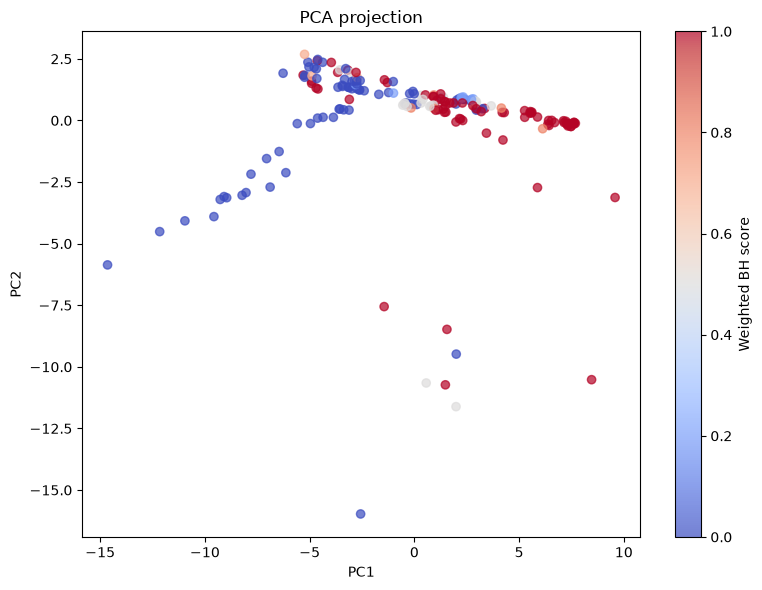
\includegraphics[width=0.96\columnwidth]{figures/pca_projection.png}
\caption{Proyección PCA de las 44 propiedades anteriores al colapso. El color muestra el puntaje BH ponderado después de ajustar PCA.}
\label{fig:pca}
\end{figure}

\subsection{Red neuronal y validación}
Se utilizó una red completamente conectada con 44 entradas, capas ocultas ReLU y una salida escalar. La salida cruda, $z_i=f_{\theta}(x_i)$, es un logit que puede tomar cualquier valor real. Se transforma mediante $\hat{s}_i=\sigma(z_i)$ para obtener el puntaje predicho. Se entrenó en PyTorch \cite{pytorch} con Adam, tasa de aprendizaje 0,001 y el conjunto completo de cada fold como lote. La función \texttt{BCEWithLogitsLoss} combina la transformación sigmoide con la entropía cruzada binaria de forma numéricamente estable. Admite el objetivo fraccionario $s_i$ de la Ec.~\eqref{eq:target}:
\begin{equation}
\mathcal L_{\mathrm{BCE}}=-\frac{1}{n}\sum_{i=1}^{n}
\left[s_i\log\hat{s}_i+(1-s_i)\log(1-\hat{s}_i)\right].
\end{equation}
Para objetivos intermedios, incluso una predicción igual al objetivo puede dar una BCE positiva. Por eso se comparan los valores entre modelos y no se interpreta cero como una meta alcanzable para todos los casos.

La selección se hizo con Leave-One-Out sobre las 140 estrellas de entrenamiento. Cada una de las 140 iteraciones ajustó el escalador y la red con 139 estrellas y evaluó la restante. Se probaron nueve arquitecturas en 50, 100, 150 y 200 épocas, para un total de 36 configuraciones. Después se extendieron cinco arquitecturas a 500 épocas para observar sus curvas de pérdida. La selección se basó en la BCE media de validación.

Además de BCE, se informan MAE (error absoluto medio), RMSE (raíz del error cuadrático medio) y $R^2$ (comparación con predecir la media del objetivo).

Se usaron pandas y NumPy \cite{pandas,numpy}, scikit-learn \cite{sklearn} y Matplotlib \cite{matplotlib}.

\section{Resultados y discusión}
\subsection{Estructura de los progenitores}
Entre las ocho propiedades examinadas en detalle, las correlaciones más altas con el puntaje BH fueron las de la compactación del núcleo (0,63) y la densidad en escala logarítmica (0,60). Ambas toman como referencia la región interior que encierra 2,5 masas solares. Las masas de los núcleos de helio y CO tuvieron correlaciones de 0,52, y la masa inicial de 0,21. Son asociaciones observadas en esta muestra y no indican por sí solas qué variables usa más la red.

En la Fig.~\ref{fig:pca}, puntajes NS y BH tienden a ocupar regiones distintas de la primera componente, aunque también se superponen. La Fig.~\ref{fig:kmeans} muestra los cinco grupos de $k$-means++ sobre esa misma proyección. La Tabla~\ref{tab:clusters} compara su composición: el grupo 1 reunió 31 estrellas con consenso BH entre 32 integrantes y el grupo 2 reunió 14 con consenso NS entre 14 integrantes. Los demás grupos mezclaron puntajes. Hay estructura en las propiedades físicas, pero no una separación completa.

\begin{figure}[!t]
\centering
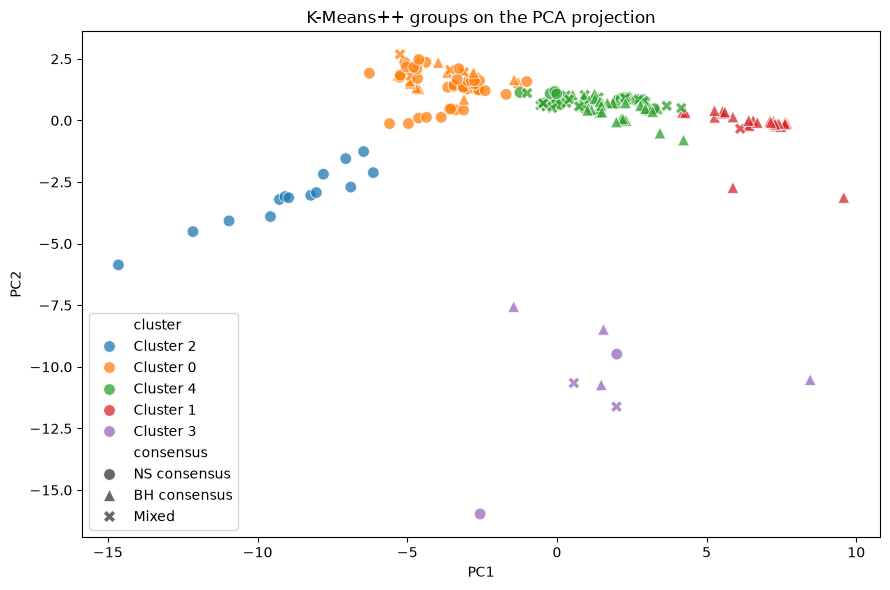
\includegraphics[width=0.96\columnwidth]{figures/kmeans_five_clusters.png}
\caption{Cinco grupos de $k$-means++ sobre PCA. El color indica el grupo y la forma indica consenso NS, BH o mixto.}
\label{fig:kmeans}
\end{figure}

\begin{table}[!t]
\caption{Composición de los cinco grupos de $k$-means++.}
\label{tab:clusters}
\centering
\begin{tabular}{rrrrr}
\toprule
Grupo & Estrellas & NS & BH & Mixto \\
\midrule
0 & 58 & 39 & 13 & 6 \\
1 & 32 & 0 & 31 & 1 \\
2 & 14 & 14 & 0 & 0 \\
3 & 8 & 2 & 4 & 2 \\
4 & 75 & 19 & 27 & 29 \\
\bottomrule
\end{tabular}
\end{table}

\subsection{Selección de arquitectura}
La grilla inicial favoreció 32 neuronas y 150 épocas (BCE media 0,4141). Al extender esta red a 500 épocas, el mínimo fue 0,4132 en la época 132. La Tabla~\ref{tab:arquitecturas} resume los mínimos de las cinco arquitecturas. La Fig.~\ref{fig:curva} muestra que después de la época 132 la pérdida de entrenamiento baja mientras la de validación sube. Por ello se fijaron 32 neuronas y 132 épocas para el entrenamiento final.

\begin{table}[!t]
\caption{Mínimo de BCE media Leave-One-Out en 500 épocas.}
\label{tab:arquitecturas}
\centering
\begin{tabular}{lrr}
\toprule
Neuronas ocultas & Época & BCE validación \\
\midrule
32 & 132 & 0,4132 \\
64 & 70 & 0,5231 \\
64--32 & 78 & 0,4660 \\
64--32--8 & 71 & 0,4896 \\
64--32--16--8 & 82 & 0,4815 \\
\bottomrule
\end{tabular}
\end{table}

\begin{figure}[!t]
\centering
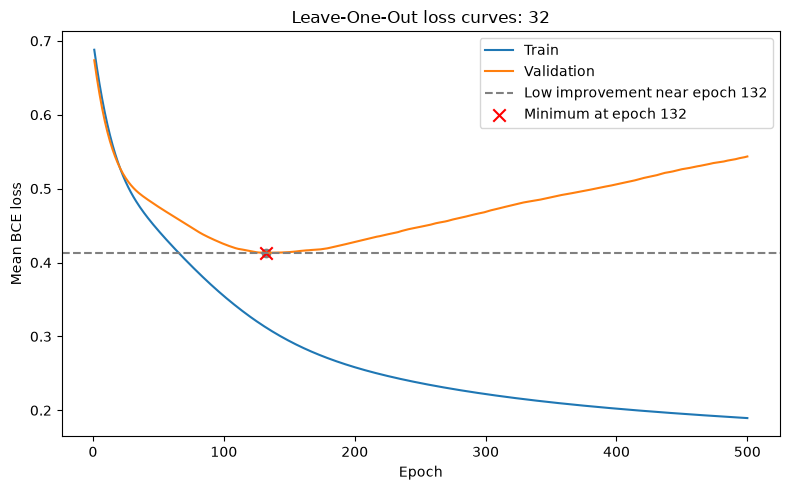
\includegraphics[width=0.98\columnwidth]{figures/validation_curves_32.png}
\caption{Curvas BCE de la red con 32 neuronas. La cruz marca el mínimo de validación en la época 132.}
\label{fig:curva}
\end{figure}

\subsection{Evaluación final}
La red elegida se entrenó otra vez con las 140 estrellas de entrenamiento y se evaluó en las 47 reservadas. Obtuvo BCE 0,3605, MAE 0,1998, RMSE 0,2726 y $R^2=0,6376$. El MAE equivale a un error absoluto medio cercano a 0,20 en la escala de cero a uno del objetivo. El $R^2$ positivo indica un error cuadrático menor que el de predecir siempre el puntaje medio. En Leave-One-Out, $R^2$ fue 0,5902. La Fig.~\ref{fig:test} muestra puntajes bajos cuando el objetivo indica NS y altos cuando indica BH, aunque algunos casos quedan lejos de la diagonal.

\begin{figure}[!t]
\centering
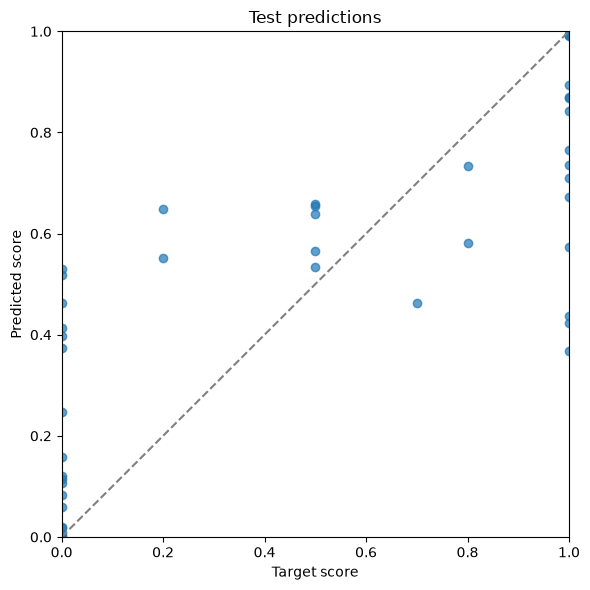
\includegraphics[width=0.88\columnwidth]{figures/test_predictions.png}
\caption{Puntajes predichos para las 47 estrellas de prueba. La diagonal representa igualdad entre predicción y objetivo.}
\label{fig:test}
\end{figure}

Como análisis exploratorio se transformaron los puntajes en etiquetas. Se asignó BH a valores mayores o iguales que 0,5 y NS a los menores. Un objetivo de 0,5 indica empate ponderado entre engines, que se resolvió como BH por convención. La red no se entrenó con estas etiquetas binarias. La precisión mide los aciertos entre las predicciones de una clase, el recall mide cuántos casos de esa clase se recuperan y F1 combina ambas medidas. Con esa convención, 39 de 47 etiquetas de prueba coincidieron. La Tabla~\ref{tab:confusion} muestra 16 NS y 23 BH correctos, con cuatro errores de cada tipo. La precisión, el recall y el F1 fueron 0,80 para NS y 0,85 para BH. La exactitud total fue 0,83. Estas métricas dependen del umbral y de cómo se resuelve el puntaje 0,5, por lo que la evaluación principal sigue siendo la del puntaje continuo.

\begin{table}[!t]
\caption{Matriz de confusión de las 47 estrellas reservadas.}
\label{tab:confusion}
\centering
\begin{tabular}{lrr}
\toprule
 & Pred. NS & Pred. BH \\
\midrule
Objetivo NS & 16 & 4 \\
Objetivo BH & 4 & 23 \\
\bottomrule
\end{tabular}
\end{table}

\section{Conclusión y trabajo futuro}
Las propiedades anteriores al colapso permitieron aproximar el consenso ponderado de los cuatro engines. En las 47 estrellas reservadas, el error absoluto medio fue cercano a 0,20 en una escala de cero a uno y $R^2$ fue 0,6376. Sin embargo, hubo errores individuales grandes. El análisis no supervisado también mostró grupos con predominio NS o BH, pero sin separación completa.

El objetivo procede de simulaciones y de pesos definidos en este trabajo, no de destinos observados. Por eso, el puntaje predicho no es una probabilidad física calibrada para una estrella real. Como trabajo futuro se podrían evaluar otros conjuntos de progenitores y estudiar qué propiedades influyen más en las predicciones.

\begin{thebibliography}{00}
\bibitem{sukhbold} T. Sukhbold, T. Ertl, S. E. Woosley, J. M. Brown y H.-T. Janka, ``Core-Collapse Supernovae from 9 to 120 Solar Masses Based on Neutrino-Powered Explosions'', \emph{The Astrophysical Journal}, vol. 821, art. 38, 2016, doi: 10.3847/0004-637X/821/1/38.
\bibitem{pytorch} A. Paszke \emph{et al.}, ``PyTorch: An Imperative Style, High-Performance Deep Learning Library'', en \emph{Advances in Neural Information Processing Systems 32}, 2019.
\bibitem{sklearn} F. Pedregosa \emph{et al.}, ``Scikit-learn: Machine Learning in Python'', \emph{Journal of Machine Learning Research}, vol. 12, pp. 2825--2830, 2011.
\bibitem{pandas} W. McKinney, ``Data Structures for Statistical Computing in Python'', en \emph{Proc. 9th Python in Science Conference}, pp. 56--61, 2010, doi: 10.25080/Majora-92bf1922-00a.
\bibitem{numpy} C. R. Harris \emph{et al.}, ``Array Programming with NumPy'', \emph{Nature}, vol. 585, pp. 357--362, 2020, doi: 10.1038/s41586-020-2649-2.
\bibitem{matplotlib} J. D. Hunter, ``Matplotlib: A 2D Graphics Environment'', \emph{Computing in Science \& Engineering}, vol. 9, no. 3, pp. 90--95, 2007, doi: 10.1109/MCSE.2007.55.
\end{thebibliography}

\end{document}
